\documentclass[10pt]{beamer}
\usetheme{AAUsimple}

\usepackage[utf8]{inputenc}
\usepackage[T1]{fontenc}
\usepackage[danish]{babel}
\usepackage{helvet}
\usepackage{listings}

\newcommand{\chref}[2]{%
  \href{#1}{{\usebeamercolor[bg]{AAUsimple}#2}}%
}


\author{}
\institute{
  Institut for Matematiske Fag\\
  Aalborg Universitet\\
  Danmark

}
\pgfdeclareimage[height=1.5cm]{titlepagelogo}{AAUgraphics/aau_logo_new}
\titlegraphic{\pgfuseimage{titlepagelogo}}


\title{Introduktion til \LaTeX}
\subtitle{Workshop 1}
\date{4. september 2019}

\begin{document}

% Title page
{\aauwavesbg
  \begin{frame}[plain,noframenumbering]
  \titlepage
\end{frame}}

% Table of contents
\begin{frame}{Agenda}{}
\tableofcontents
\end{frame}

% Main content
\section{Introduktion}
\begin{frame}{Introduktion}
  Hvad er \LaTeX, og hvorfor er det nødvendigt at kende til som matematikstuderende?
  \begin{itemize}
  \item \LaTeX er et typografisk system som blandt andet er særligt velegnet til at skrive matematiske formler.
  \item Det er IKKE et WYSIWYG program ligesom Microsoft Word etc.
  \item Tekst og formler skrives i et kodesprog som først bliver \emph{kompileret}, hvorefter der dannes en pdf med resultatet.
  \item Ekstra funktionalitet kan tilføjes med \emph{pakker}, og man kan skrive sine egne kommandoer/funktioner
  \item Det kræver tilvænning at skrive i \LaTeX; fejl i ens kode vil medføre \emph{kompileringsfejl}, som skal rettes for at en pdf kan dannes.
  \end{itemize}
\end{frame}

\begin{frame}[containsverbatim]{Introduktion}{Hello World!}
  \begin{block}{master.tex}
\begin{verbatim}
  \documentclass[10pt]{article}
  \begin{document}
  Hello World! I present to you Eulers identity:
  \begin{equation}
    \label{eq:eulers_identity}
    e^{i\pi} + 1 = 0.
  \end{equation}
  \end{document}
\end{verbatim}
  \end{block}
  \begin{block}{master.pdf}
    Hello World! I present to you Eulers identity:
    \begin{equation}
      \label{eq:eulers_identity}
      e^{i\pi} + 1 = 0.
    \end{equation}
  \end{block}
\end{frame}

\section{Mappestruktur og Filtyper}
\begin{frame}[containsverbatim]{Mappestruktur og Filtyper}{Mappestruktur}
  Det er en god ide at have en ordnet mappestruktur på sin computer.
  \begin{tikzpicture}
    \draw[color=black!60!white]
    \FTdir(\FTroot,root,Documents){
      \FTdir(root,AAU,AAU){
        \FTdir(AAU,semester1,semester1){
          \FTdir(semester1,P0,P0) {}
          \FTdir(semester1,P1,P1) {}
          \FTdir(semester1,LIAL,LIAL) {}
          \FTdir(semester1,intro,\LaTeX-intro) {}
        }
        \FTdir(AAU,semester2,semester2){
          \FTdir(semester2,P2,P2) {}
          \FTdir(semester2,CALC,CALC) {}
        }
      }
    };
  \end{tikzpicture}
\end{frame}

\begin{frame}{Mappestruktur og Filtyper}{Filtyper}
  Der findes mange forskellige filtyper og det er en fordel at have hørt om de mest almindelige.

  \begin{block}{}
    \begin{tabular}{ll}
      \texttt{.txt}  & Plain tekst \\
      \texttt{.docx} & Microsoft Word \\
      \texttt{.csv}  & ``Comma Separated Values''; tabel-data \\
      \texttt{.pdf}  & ``Portable Document Format''; read-only dokumentformat \\
      \texttt{.jpeg} & Billedformat \\
      \texttt{.png}  & Billedformat \\
      \texttt{.html} & Hjemmesideformat \\
      \texttt{.zip}  & Arkivfil \\
      \texttt{.tex}  & \LaTeX-fil \\
      \texttt{.bib}  & Bibliografifil (hørende til \LaTeX)
    \end{tabular}
  \end{block}
\end{frame}

\begin{frame}{Mappestruktur og Filtyper}{.zip filer}
  Hvis man har brug for, at dele mange mapper og filer med andre kan det være en god ide at komprimere disse til en enkelt \texttt{.zip}.
  \begin{block}{Windows}
    I Windows kan man markere de filer og mapper man vil komprimere, derefter højreklikke og trykke
    \begin{itemize}
    \item \texttt{Send til} $\to$ \texttt{Kromprimeret (zip) mappe}.
    \end{itemize}
  \end{block}

  \begin{block}{macOS}
    I macOS skal man markere de filer og mapper man vil komprimere, derefter højreklikke og trykke
    \begin{itemize}
    \item \texttt{Kromprimer}.
    \end{itemize}
  \end{block}
\end{frame}

\section{TeXMaker}

\begin{frame}
  \frametitle{TeXMaker}
  \framesubtitle{Redigeringsprogram til \LaTeX}
  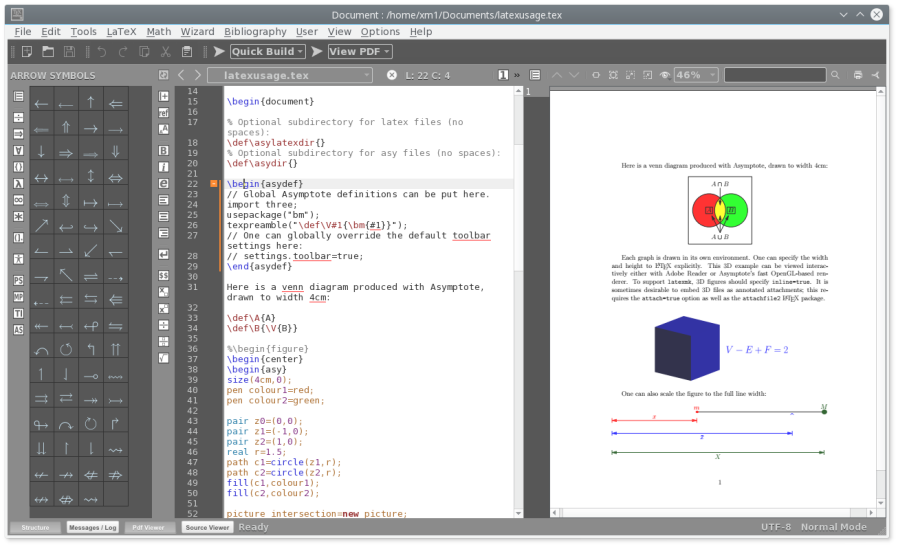
\includegraphics[width=\textwidth]{img/texmaker.png}
\end{frame}

\begin{frame}
  \frametitle{TeXMaker}
  \framesubtitle{Redigeringsprogram til \LaTeX}

  \begin{block}{\chref{https://www.xm1math.net/texmaker}{https://www.xm1math.net/texmaker}}
    \begin{itemize}
    \item Begyndervenlig editor til at skrive {\LaTeX} i
    \item Tilgængelig på GNU/Linux, macOS og Windows
    \item Fri software
    \end{itemize}
  \end{block}

  \begin{block}{Alternativer}
    \begin{itemize}
    \item TeXStudio (\chref{https://www.texstudio.org}{https://www.texstudio.org})
    \item Atom (\chref{https://atom.io}{https://atom.io})
    \item Emacs (\chref{https://www.gnu.org/software/emacs}{https://www.gnu.org/software/emacs})
    \item Hvilken som helst plain text editor
    \end{itemize}
  \end{block}
\end{frame}

\section{Must Know \LaTeX \ \ Kommandoer}

\begin{frame}{Must Know \LaTeX \ Kommandoer}{Specielle karakterer}
  \begin{table}[h]
    \centering
    \begin{tabular}[h]{llll}
      \textbf{Tegn}             & \textbf{Beskrivelse} & \textbf{Eksempel} & \textbf{Resultat}\\ \hline \\[2pt]
      \texttt{\textbackslash}   & begynd kommando      & \texttt{\textbackslash LaTeX}              & \LaTeX        \\[4pt]
      \texttt{\{ \}}            & omkrans argumenter   & \texttt{\textbackslash textbf\{fed\}}    & \textbf{fed}  \\[4pt]
      \texttt{\%}               & kommentar tegn       & \texttt{\% Fix}                            & \% Fix        \\[4pt]
      \texttt{\$ \$}            & inline matematik     & \texttt{\$\textbackslash frac\{1\}\{2\}\$} & $\frac{1}{2}$ \\[4pt]
      \texttt{\_}               & subscript            & \texttt{\$x\_i\$}                          & $x_i$         \\[4pt]
      \texttt{\textasciicircum} & superscript          & \texttt{\$x\textasciicircum 2\$}           & $x^2$
    \end{tabular}
  \end{table}
\end{frame}

\begin{frame}[containsverbatim]{Must Know \LaTeX \ Kommandoer}{Blokmiljøer}
  Et blokmiljøe (engelsk: environment) udfører en handling på en blok af kommandoer i modsætning til eksempelvis inline matematik ved brug af \$ \$.
  \begin{block}{Form}
\begin{verbatim}
  \begin{miljø}
  ...
  ...
  \end{miljø}
\end{verbatim}
  \end{block}
\end{frame}

\section{Matematik Specifikt}

\begin{frame}[fragile,label = mustknow]{Matematik Specifikt}
  \begin{block}{Blokmiljøer}
\begin{verbatim}
 \begin{equation} ... \end{equation}
 \begin{align}    ... \end{align}
 \begin{pmatrix}  ... \end{pmatrix}
 \begin{cases}    ... \end{cases}
\end{verbatim}
\end{block}

\begin{block}{Andet}
\begin{verbatim}
 \sum_{i = 1}^{n} x_i
 \prod_{i \in \mathcal{I}}p(i)
 \int_{\infty}^{infty} f(x)dx
 \frac{d}{dx}f(x)
\end{verbatim}
\end{block}

Se også: \href{https://en.wikibooks.org/wiki/LaTeX/Mathematics}{Wiki - Mathematics}
\end{frame}

\section{Opgaver}

\begin{frame}[containsverbatim]{Opgaver}{Opgave 1}
  \begin{itemize}
  \item Lave en AAU mappestruktur
  \item Dan en undermappe \texttt{latex-p0}
  \item Opret filen \texttt{hello\textunderscore world.tex}
  \item Skriv følgende i filen og compiler dokumentet
  \end{itemize}

  \begin{block}{hello\textunderscore world.tex}
\begin{verbatim}
  \documentclass[10pt]{article}
  \begin{document}
   Hello World! I Like Mathematics!
  \end{document}
\end{verbatim}
  \end{block}  

\end{frame}

\begin{frame}[containsverbatim]{Opgaver}{Opgave 2}
  \begin{itemize}
  \item Brug linket på slide \ref{mustknow} til at genskabe nedenstående
  \end{itemize}
  \begin{block}{}
    \begin{align*} 
      \pi          &= \frac{O}{D} \\
      e^{i\pi} + 1 &= 0           \\
      \frac{\partial^2 u}{\partial t^2} & = c^2 \nabla^2 u \\
      P_k(x) &= \sum_{i=1}^{k} \frac{f^{(k)}(a)}{k!}(x - a)^k
    \end{align*}
  \end{block}
\end{frame}


\end{document}

%%% Local Variables:
%%% mode: latex
%%% TeX-master: t
%%% End:
